\section{Results}

\subsection{Stability of Hopfield Network}
\begin{figure}[H]
    \centering
    \begin{subfigure}{0.49\textwidth}
        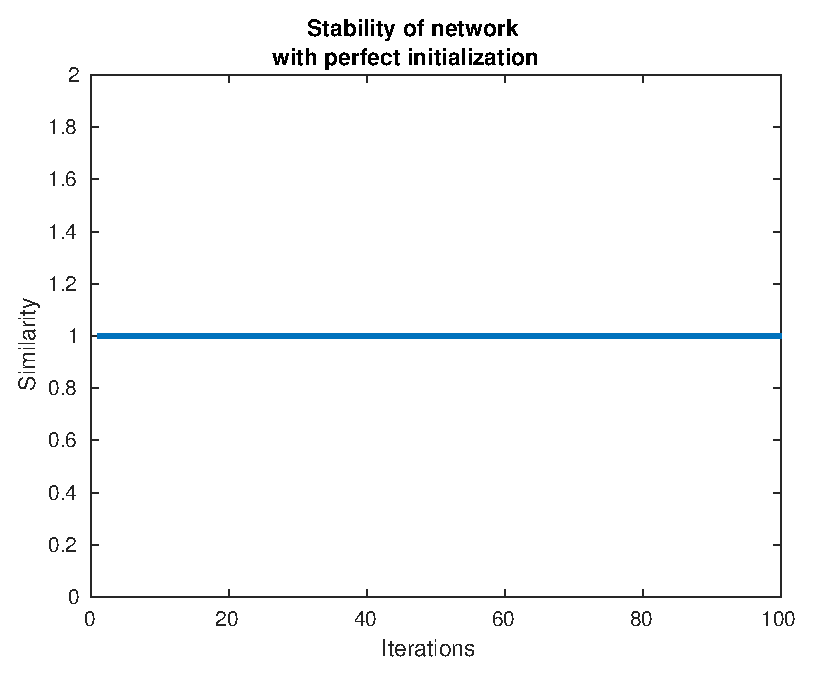
\includegraphics[width=\textwidth]{figs/stable}
        \caption{By initializing the network to the stored pattern, the network will remain in an equilibrium. The network will never deviate from this state without external interference.}
    \end{subfigure}
    \begin{subfigure}{0.49\textwidth}
        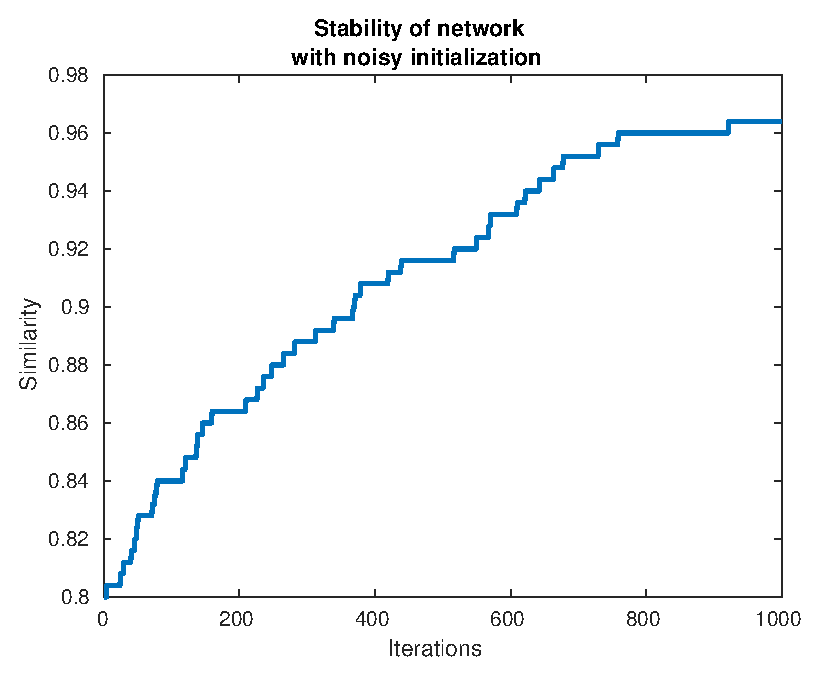
\includegraphics[width=\textwidth]{figs/stable-with-noise}
        \caption{If the network is initialized to a noisy state, the network will converge towards the stored pattern. }
    \end{subfigure}
    \caption{Initializing a Hopfield network with a single stored pattern will cause the network to converge towards the stored pattern.}
\end{figure}
To test whether the Hopfield network is indeed stable, we simulated a 

\subsection{Storing multiple patterns}
\begin{figure}[H]
    \centering
    \begin{subfigure}{0.49\textwidth}
        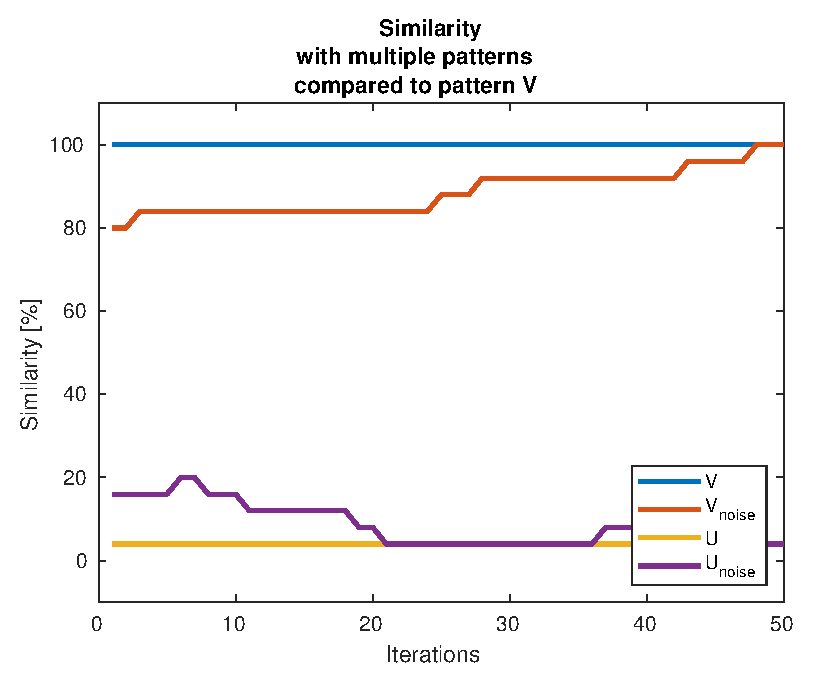
\includegraphics[width=\textwidth]{figs/multiple-patterns.eps}
        \caption{By initializing the weight matrix $\bf W$ with multiple patterns, the network is able to restore multiple different patterns. The amount of memories and noise the network is able to handle, depends on complex the pattern is (number of neurons) and how similar the patterns are. If two stored patterns only differ by one bit, the network may recall the wrong memory if noise is involved. }
    \end{subfigure}
    \begin{subfigure}{0.49\textwidth}
        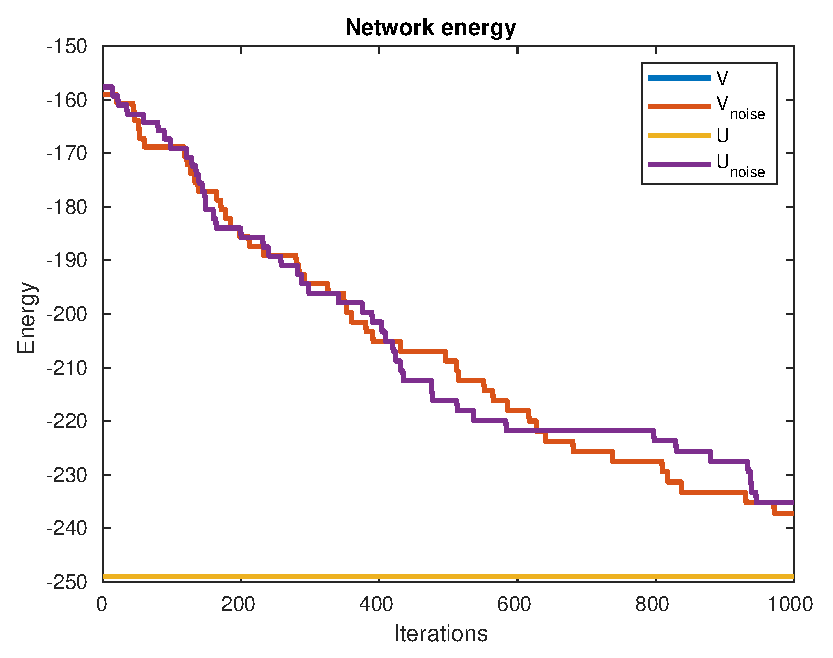
\includegraphics[width=\textwidth]{figs/multiple-patterns-energy.eps}
        \caption{The network will always move in the direction of least resistance such that the overall energy decrease, similar to how a ball always will roll downwards into a valley unless there are external forces interfering. Each stored memory corresponds to a local minimum which can be thought of as valleys, and as long as the network is initialized in the correct valley, it is able to reconstruct the state from memory.}
    \end{subfigure}
\end{figure}
 

\subsection{Reconstructing partially lost QR codes from memory} \label{sec:qr-codes}
To better visualize the Hopfield networks ability to store and restore patterns, we constructed a Hopfield network to store QR-codes. We stored two QR-codes in the network and initialized the network with only partial information. \cref{fig:qr-codes} shows how the network was able to restore the correct QR code from memory, while \cref{fig:qr-codes-stability} shows how the network remains stable after reaching the equilibrium.
\begin{figure}[H]
    \centering
    \begin{subfigure}{0.49\textwidth}
        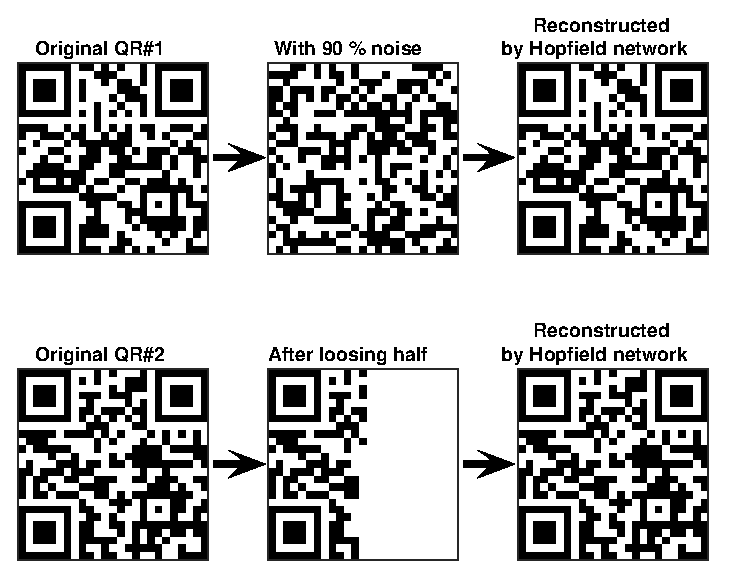
\includegraphics[width=\textwidth]{figs/qr-code}
        \caption{The QR-code contains information encoded within the patterns. A QR decoding app, either online or on a smartphone, can be used to decode the "hidden" message. Using the hopfield network we are able to reconstruct a destroyed QR-code from memory.}
        \label{fig:qr-codes}
    \end{subfigure}
    \begin{subfigure}{0.49\textwidth}
        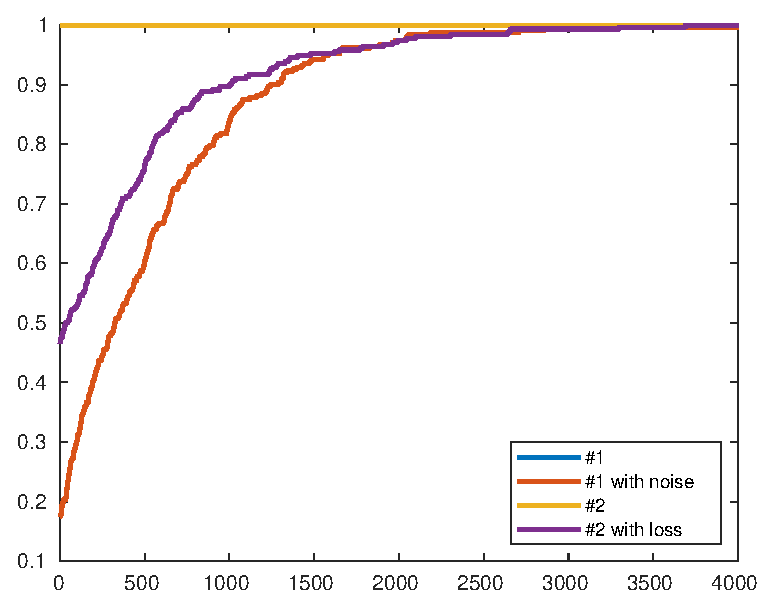
\includegraphics[width=\textwidth]{figs/qr-code-sim}
        \caption{The similarity between the current state of the network and the original QR-code we want it to reconstruct.}
        \label{fig:qr-codes-stability}
    \end{subfigure}
    \caption{By applying the Hopfield network to a very noisy QR-code we are able to reconstruct the original. By using any QR-code reader we are able to decode the left and right QR-codes, while the middle ones contains too much noise. The same hopfield network was used.}
\end{figure}

\subsection{Inverting patterns}
According to the weights, \cref{eq:weights}, the Hopfield network only stores patterns and not the actual values in the memories. A pattern $\bf V$ and its inverse $\bf \bar{V} = -1 \times \bf V$ would yield the exact same weight matrix. For each stored memory there should be two equilibrium states, one for $\bf V$ and one for $\bf \bar{V}$. To test wheter this truly was the case, we used the same Hopfield network as in \cref{sec:qr-codes} and initialized the states to the second QR code, but inverted. We ran another simulation using the QR-code with a two-thirds of its bits inverted. As can be seen from the results in \cref{fig:inverted-qr} both cases caused the Hopfield network to reconstruct the inverted pattern, and not the one we originally created. From \cref{eq:weights} this makes sense, since we only store whether two neurons should contain the same state or not. The Hopfield network only store what the state should be relative to others in the network.
\begin{figure}[H]
    \centering
        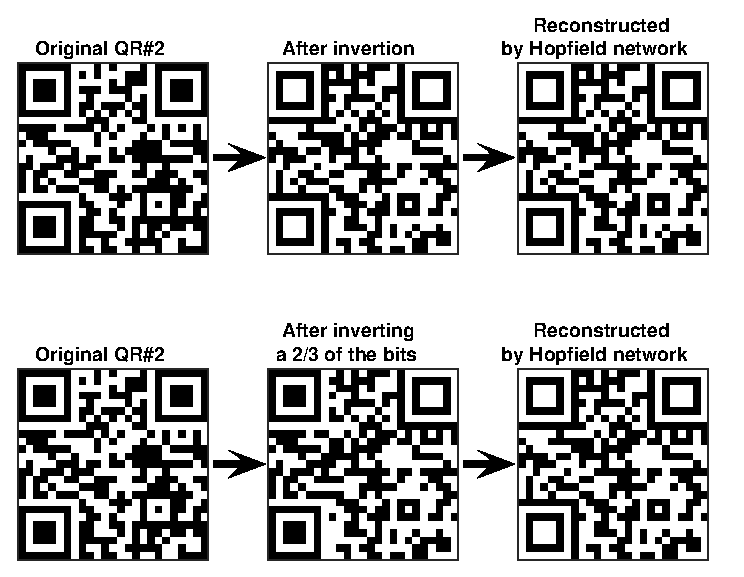
\includegraphics[width=0.4\textwidth]{figs/qr-inverted}
        \caption{The Hopfield network learns the patterns and the network is not able to distinguish between positive and negative values. The network is not only stable at the initial memories, but also when using the inverted patterns. This makes sense from a memory point of view, as we are able to distinguish objects purely based on patterns and shapes. An apple is an apple regardless of its color.}
        \label{fig:inverted-qr}
\end{figure}